\subsubsection{SEDE}

% figure sede_sql.jpg
\begin{figure}[H]
    \centering
    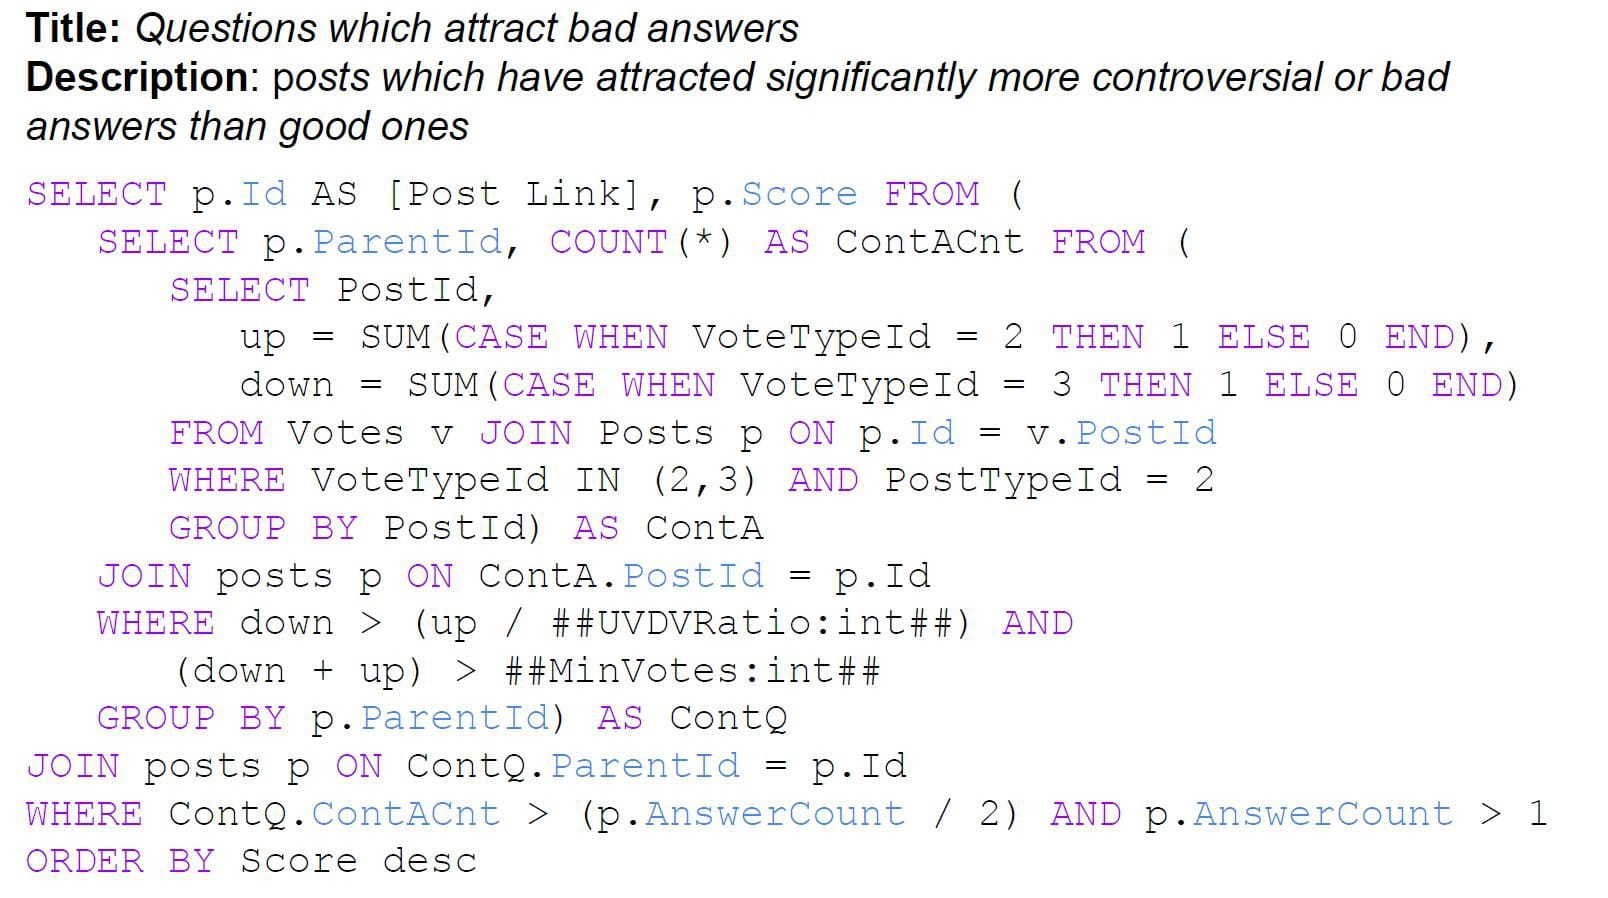
\includegraphics[width=0.8\linewidth]{pics/sede_sql.jpg}
    \caption{An example of a Complex query from the SEDE dataset.\cite{DBLP:journals/corr/abs-2106-05006}}
    \label{fig:sede_sql}
\end{figure}

\ac{SEDE} \cite{DBLP:journals/corr/abs-2106-05006} is from a popular online question-and-answer platform with more than 3 million questions, and it recently released a benchmark dataset of SQL queries containing 29 tables and 211 columns. This dataset comprises real-world questions from the Stack Exchange website, such as published posts, comments, votes, tags, and awards.

Although these datasets contain a variety of real-world challenges, they still need to be more tricky to parse semantically due to the complexity of the questions they contain. After further analysis of the 12,023 questions (clean) asked on the platform, a total of 1,714 have been verified by humans, which makes it an ideal choice for training and validating the model. This benchmark dataset is highly valuable and helpful for research in natural language processing, as it provides an extensive list of real-world challenges that have rarely been seen in other semantic parsing datasets.